\documentclass[a4paper, 11pt]{scrartcl}
\usepackage[T1]{fontenc}
\usepackage[utf8]{inputenc}
\usepackage[english]{babel}
\usepackage[a4paper, margin=25mm]{geometry}
\usepackage{microtype}
\usepackage{graphicx}
\usepackage{tabularray}
\usepackage{booktabs}
\usepackage{siunitx}
\usepackage[hidelinks]{hyperref}

\title{DLS Analysis Report}
\author{}
\date{\today}

\begin{document}
\maketitle

\section*{Experiment Metadata}
\begin{tblr}{lX}
  \textbf{Analysis started} & 2026-06-09 16:57:32 \\
  \textbf{JADE-DLS version} & 2.0 \\
  \textbf{Angles} & 30°, 40°, 50°, 60°, 70°, 80°, 90°, 100°, 110°, 120°, 130°, 140°, 150° \\
  \textbf{Temperature} & 297.94 ± 0.005 K \\
  \textbf{Viscosity} & 0.8945 cP \\
  \textbf{Files} & 39 \\
\end{tblr}

\section*{Result Details --- Method A}
\emph{2026-06-09 16:59:42}

\begin{tblr}{lllllllll}
  \SetRow{font=\bfseries} Fit & Rh [nm] & Rh error [nm] & D [m\textasciicircum{}2/s] & std err D [m\textasciicircum{}2/s] & R\_squared & Residuals & PDI & Skewness \\
  \hline
  Rh from 1st order cumulant fit & 80.1057 & 0.5473 & 3.046e-12 & 2.081e-14 & 0.9983 & Possibly not normally distributed & N/A & N/A \\
  Rh from 2nd order cumulant fit & 78.3628 & 0.4530 & 3.113e-12 & 1.800e-14 & 0.9988 & Normally distributed & 0.1142 & N/A \\
  Rh from 3rd order cumulant fit & 78.3585 & 0.4674 & 3.114e-12 & 1.857e-14 & 0.9987 & Normally distributed & 0.1314 & 0.3135 \\
\end{tblr}

\begin{tblr}{lllll}
  \SetRow{font=\bfseries} Order & Slope (D×10¹⁵ m²/s) & Std Error & R² & Quality \\
  \hline
  1st & 3045.730080 & 20.809402 & 0.998276 & ✓ Excellent \\
  2nd & 3113.470797 & 17.998126 & 0.998765 & ✓ Excellent \\
  3rd & 3113.643288 & 18.571764 & 0.998685 & ✓ Excellent \\
\end{tblr}

\section*{Result Details --- Method C}
\emph{2026-06-09 16:59:51}

\begin{tblr}{llllllllll}
  \SetRow{font=\bfseries} Rh [nm] & Rh error [nm] & D [m²/s] & D error [m²/s] & R\_squared & Fit & Residuals & PDI & Skewness & Kurtosis \\
  \hline
  78.5425 & 0.5355 & 3.106e-12 & 2.118e-14 & 0.9983 & Rh from iterative non-linear cumulant fit (4th order) & Normally distributed & 0.1158 & -5.6345 & -77.5288 \\
\end{tblr}

\begin{tblr}{ll}
  \SetRow{font=\bfseries} Model Statistics &  \\
  \hline
  R-squared & 0.998283 \\
  Adj. R-squared & 0.998237 \\
  F-statistic & 2.152e+04 \\
  Prob (F-statistic) & 9.046e-53 \\
  AIC & 368.51 \\
  BIC & 371.83 \\
\end{tblr}

\begin{tblr}{lll}
  \SetRow{font=\bfseries} Coefficient & Value & Std Error \\
  \hline
\end{tblr}

\begin{tblr}{llll}
  \SetRow{font=\bfseries} Metric & Value & Optimal Range & Assessment \\
  \hline
  R² & 0.9983 & > 0.95 (Excellent)0.90-0.95 (Acceptable)< 0.90 (Poor) & ✓ Excellent \\
  Adjusted R² & 0.9982 & > 0.95 (Excellent)0.90-0.95 (Acceptable)< 0.90 (Poor) & ✓ Excellent \\
  F-statistic & 21517.77 & > 100 (Excellent)10-100 (Acceptable)< 10 (Poor) & ✓ Excellent \\
  p-value (F-test) & 9.046e-53 & < 0.001 (Excellent)0.001-0.05 (Acceptable)> 0.05 (Poor) & ✓ Excellent \\
\end{tblr}

\begin{tblr}{llll}
  \SetRow{font=\bfseries} Moment & Value & Formula & Available for \\
  \hline
  Skewness & -5.6345 & κ₃ / κ₂\textasciicircum{}(3/2) & 3rd \& 4th order \\
  Kurtosis & -77.5288 & κ₄ / κ₂² & 4th order only \\
\end{tblr}

\begin{tblr}{llllllllll}
  \SetRow{font=\bfseries} Rh [nm] & Rh error [nm] & D [m²/s] & D error [m²/s] & R\_squared & Fit & Residuals & PDI & Skewness & Kurtosis \\
  \hline
  78.5425 & 0.5355 & 3.106e-12 & 2.118e-14 & 0.9983 & Rh from iterative non-linear cumulant fit (4th order) & Normally distributed & 0.1158 & -5.6345 & -77.5288 \\
\end{tblr}

\begin{tblr}{ll}
  \SetRow{font=\bfseries} Model Statistics &  \\
  \hline
  R-squared & 0.998283 \\
  Adj. R-squared & 0.998237 \\
  F-statistic & 2.152e+04 \\
  Prob (F-statistic) & 9.046e-53 \\
  AIC & 368.51 \\
  BIC & 371.83 \\
\end{tblr}

\begin{tblr}{lll}
  \SetRow{font=\bfseries} Coefficient & Value & Std Error \\
  \hline
\end{tblr}

\begin{tblr}{llll}
  \SetRow{font=\bfseries} Metric & Value & Optimal Range & Assessment \\
  \hline
  R² & 0.9983 & > 0.95 (Excellent)0.90-0.95 (Acceptable)< 0.90 (Poor) & ✓ Excellent \\
  Adjusted R² & 0.9982 & > 0.95 (Excellent)0.90-0.95 (Acceptable)< 0.90 (Poor) & ✓ Excellent \\
  F-statistic & 21517.77 & > 100 (Excellent)10-100 (Acceptable)< 10 (Poor) & ✓ Excellent \\
  p-value (F-test) & 9.046e-53 & < 0.001 (Excellent)0.001-0.05 (Acceptable)> 0.05 (Poor) & ✓ Excellent \\
\end{tblr}

\begin{tblr}{llll}
  \SetRow{font=\bfseries} Moment & Value & Formula & Available for \\
  \hline
  Skewness & -5.6345 & κ₃ / κ₂\textasciicircum{}(3/2) & 3rd \& 4th order \\
  Kurtosis & -77.5288 & κ₄ / κ₂² & 4th order only \\
\end{tblr}

\section*{Result Summary --- Method C}
\emph{2026-06-09 16:59:55}
\begin{tblr}{llllllll}
  \textbf{Method} & \textbf{Rh (nm)} & \textbf{Error (nm)} & \textbf{D (m²/s)} & \textbf{D err (m²/s)} & \textbf{R²} & \textbf{PDI} & \textbf{Residuals} \\
  \hline
  Method C filtered (N=27 pts, 4th order) & 78.28 & 0.61 & 3.117e-12 & 2.428e-14 & 0.9985 & 0.1216 & Normally distributed \\
\end{tblr}

\begin{figure}[htbp]
  \centering
  % 2026-06-09 17:00:06
  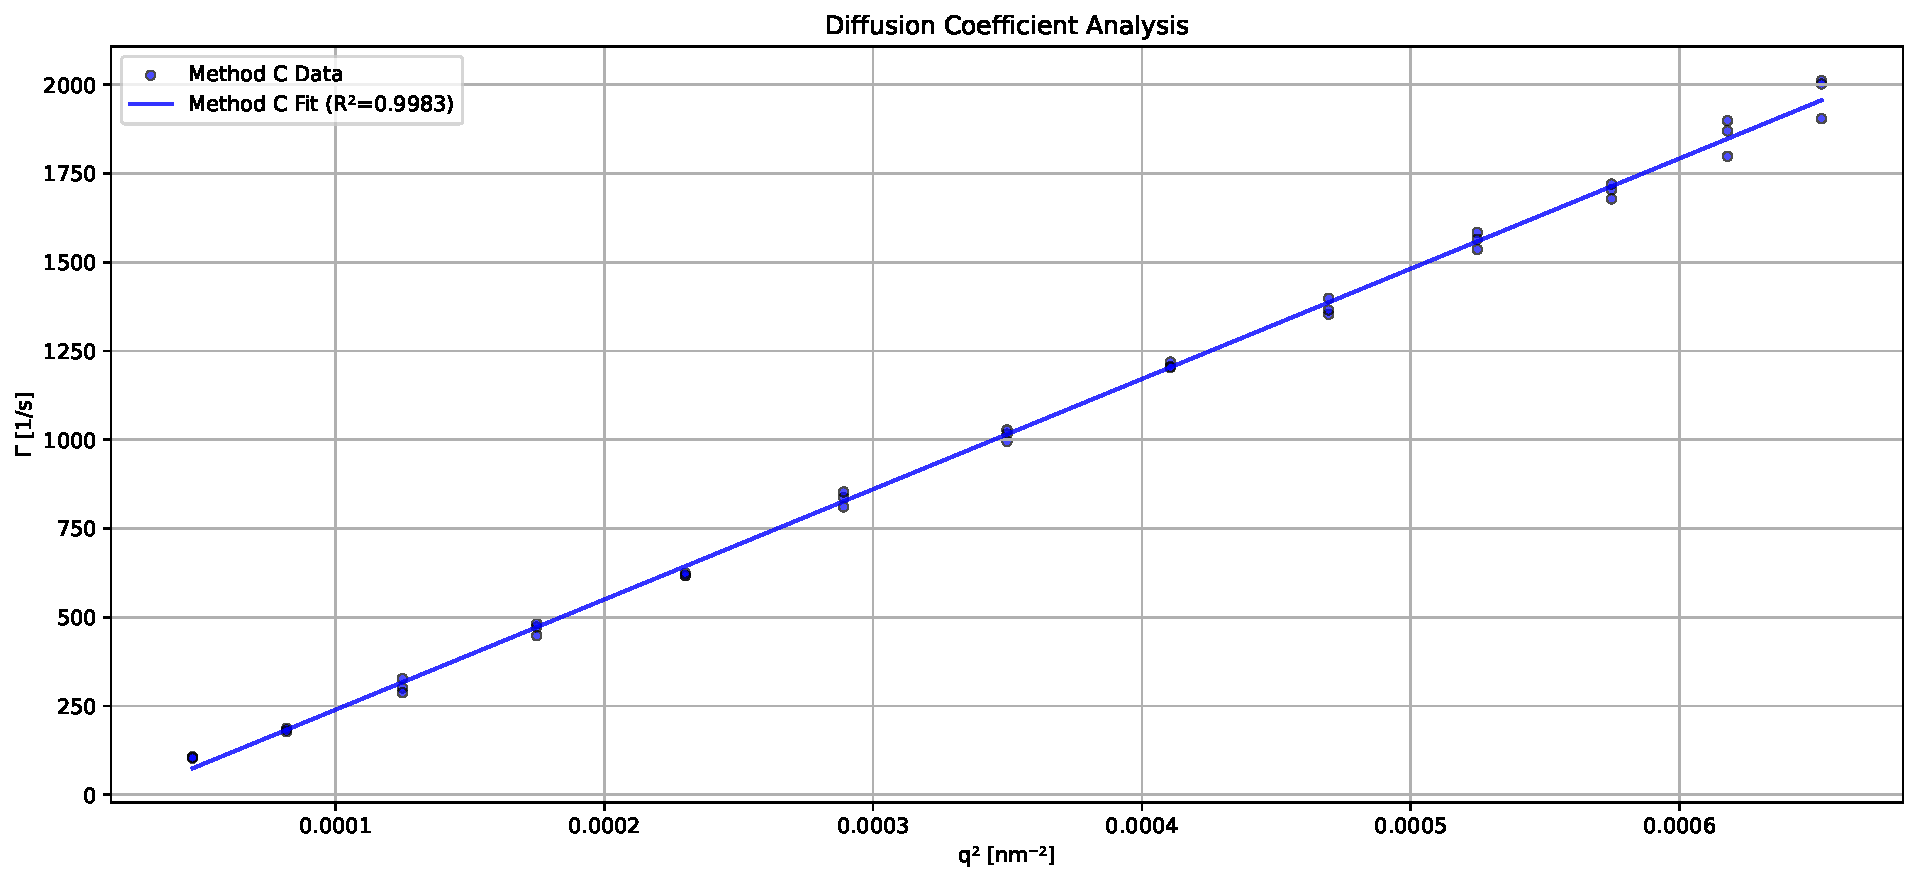
\includegraphics[width=\linewidth]{figures/plot_01_1_Method_C_Summary.pdf}
  \caption{1. Method C Summary}
  \label{fig:plot_01_1_Method_C_Summary}
\end{figure}

\begin{figure}[htbp]
  \centering
  % 2026-06-09 17:00:13
  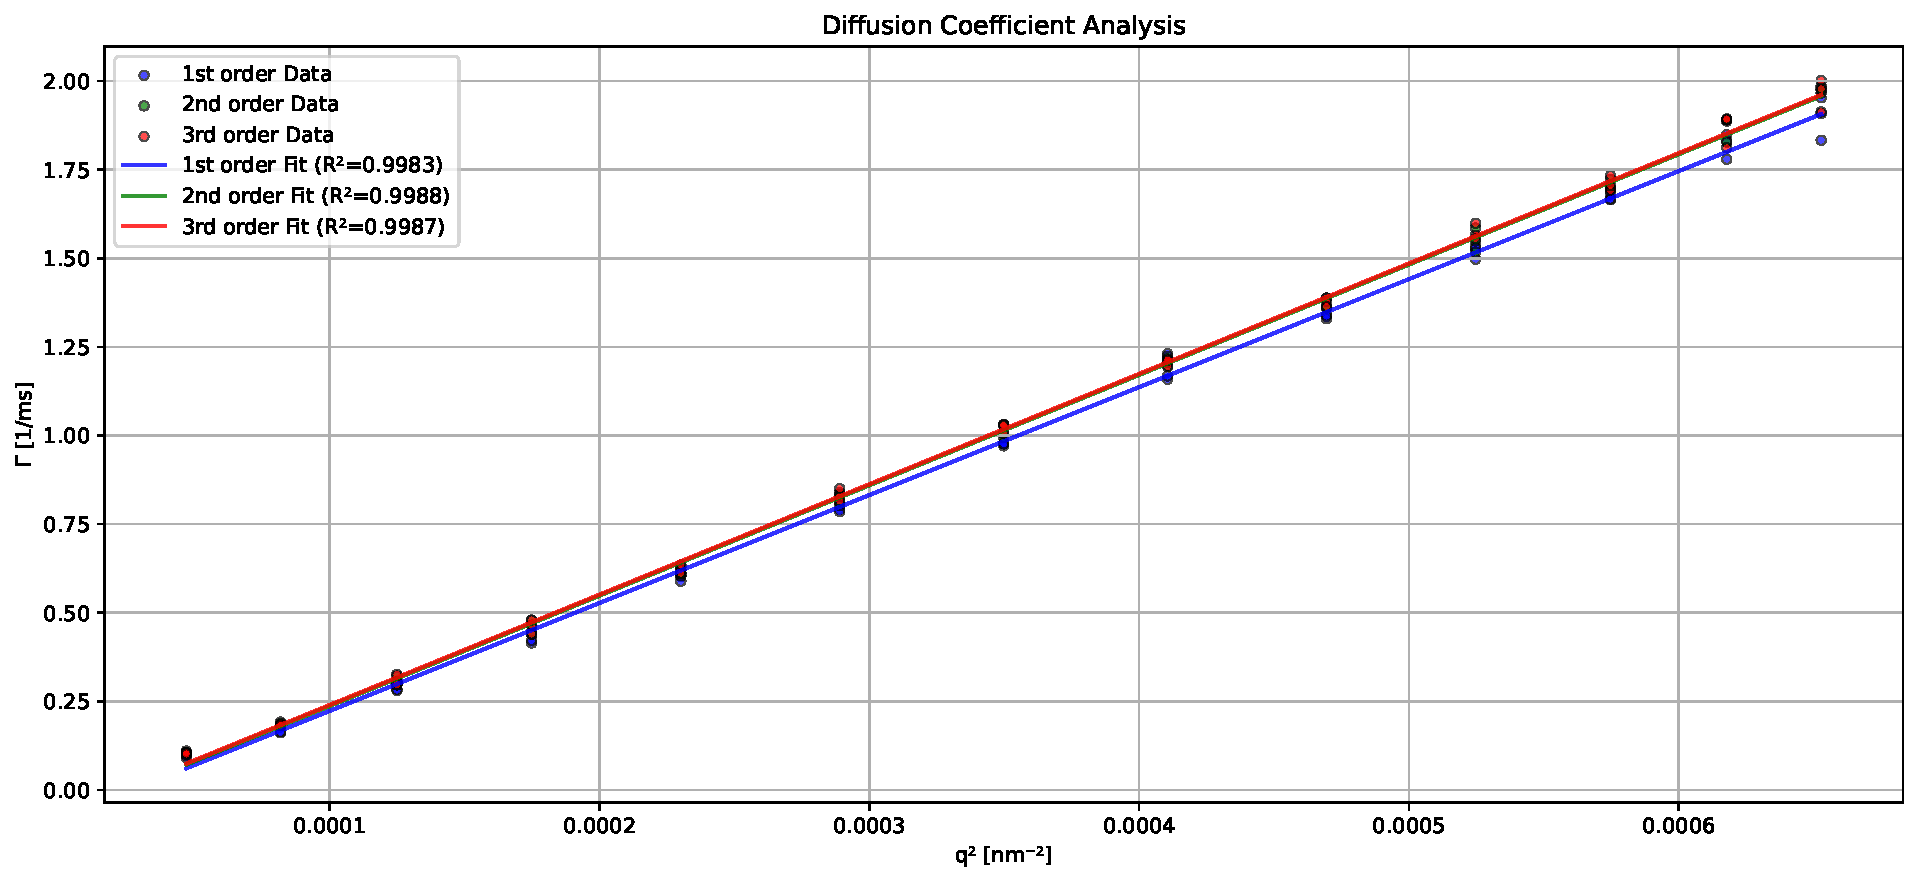
\includegraphics[width=\linewidth]{figures/plot_02_1_Method_A_Summary.pdf}
  \caption{1. Method A Summary}
  \label{fig:plot_02_1_Method_A_Summary}
\end{figure}

\section*{Result Summary --- NNLS Analysis}
\emph{2026-06-09 17:00:42}
\begin{tblr}{llllllll}
  \textbf{Method} & \textbf{Rh (nm)} & \textbf{Error (nm)} & \textbf{D (m²/s)} & \textbf{D err (m²/s)} & \textbf{R²} & \textbf{PDI} & \textbf{Residuals} \\
  \hline
  NNLS Peak 1 & 75.39 & 1.17 & nan & nan & 0.9912 & N/A & nan \\
\end{tblr}

\begin{figure}[htbp]
  \centering
  % 2026-06-09 17:01:02
  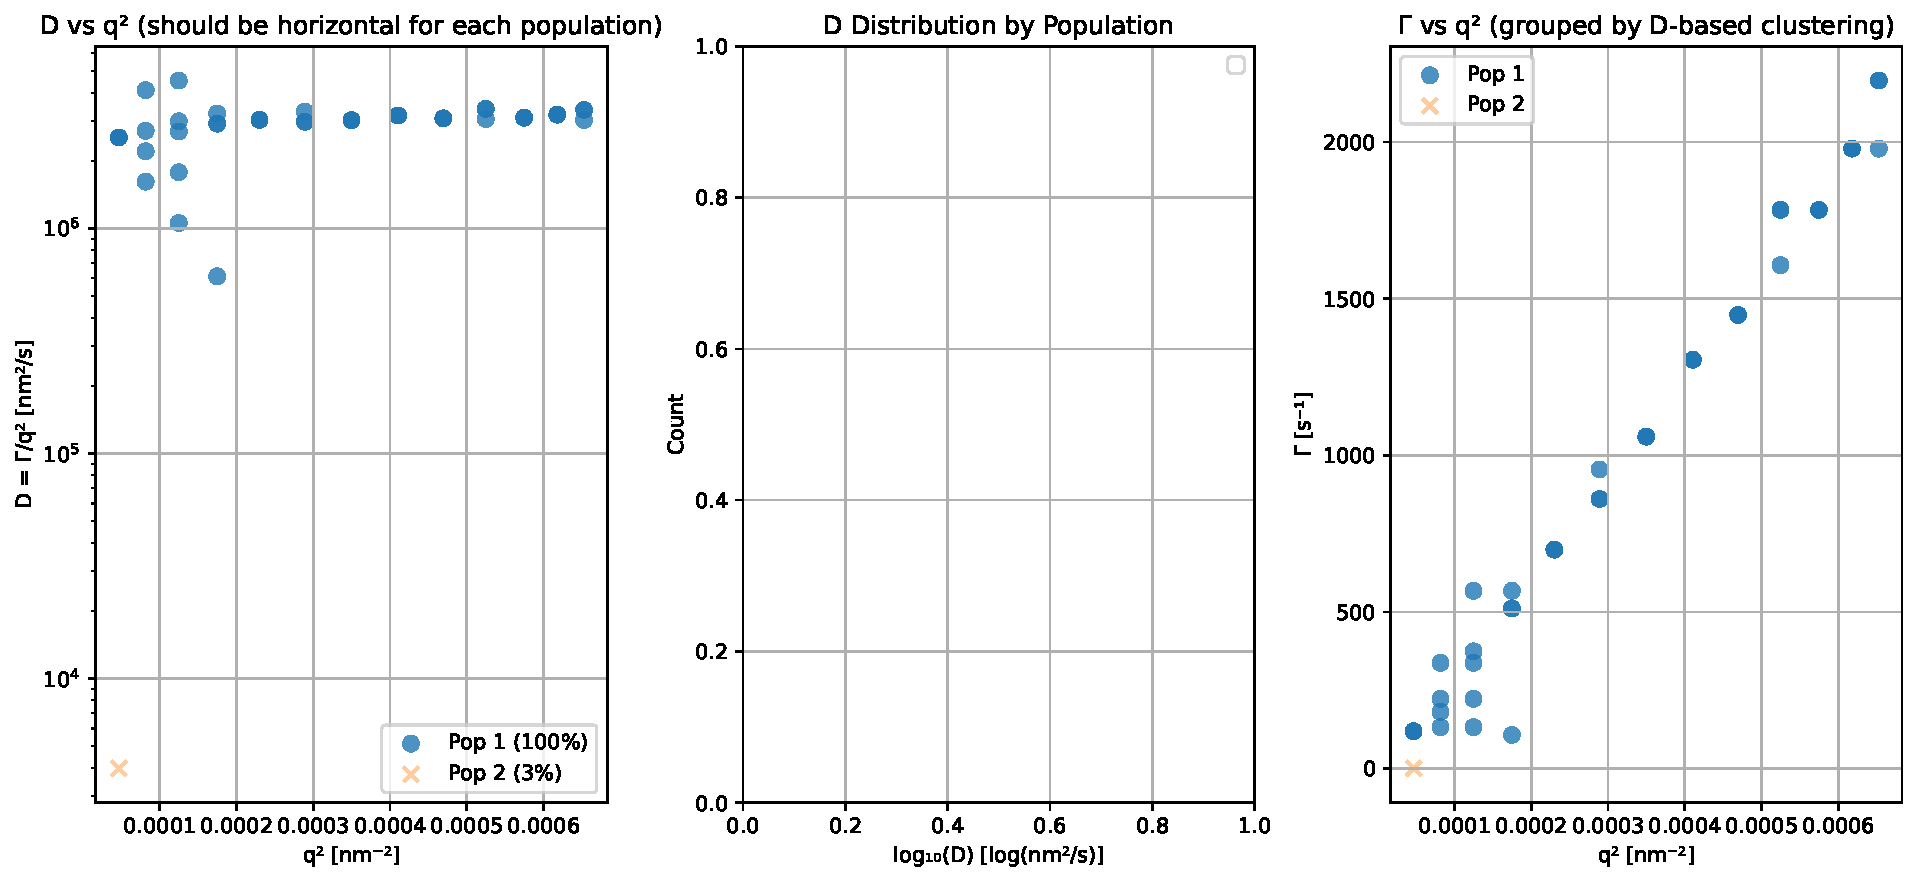
\includegraphics[width=\linewidth]{figures/plot_03_43_NNLS_Peak_Clustering.pdf}
  \caption{43. NNLS Peak Clustering}
  \label{fig:plot_03_43_NNLS_Peak_Clustering}
\end{figure}

\end{document}
